% \pagebreak[4]
% \hspace*{1cm}
% \pagebreak[4]
% \hspace*{1cm}
% \pagebreak[4]

\chapter{Tổng quan}
\ifpdf
    \graphicspath{{Chapter1/Chapter1Figs/PNG/}{Chapter1/Chapter1Figs/PDF/}{Chapter1/Chapter1Figs/}}
\else
    \graphicspath{{Chapter1/Chapter1Figs/EPS/}{Chapter1/Chapter1Figs/}}
\fi

\section{Giới thiệu bài toán}

Bài toán 8-puzzle là một bài toán trò chơi trí tuệ thường được biết với cái tên là "Xếp hình".  8-puzzle vì nó bao gồm một bảng gồm 9 ô vuông (3x3) và 8 ô vuông chứa các con số từ 1 đến 8, còn lại là 1 ô trống.
Mục tiêu của bài toán là di chuyển các ô vuông để sắp xếp các số từ 1 đến 8 vào vị trí đúng, sao cho ô trống nằm ở vị trí cuối cùng. Trong mỗi lần di chuyển, chỉ có thể đổi chỗ ô trống với một ô vuông kề cạnh nó. 
Bài toán 8-puzzle là một bài toán NP-khó, nghĩa là không có giải thuật đơn giản để giải quyết nó trong thời gian hợp lý đối với các bảng kích thước lớn. Nhiều giải thuật đã được đề xuất để giải quyết bài toán này, bao gồm giải thuật tìm kiếm theo chiều rộng (BFS), tìm kiếm theo chiều sâu (DFS), thuật toán A* và thuật toán heuristic.

\section{Điều kiện để hoàn thành}
Mỗi ô trong 8- puzzle sẽ có tối đa 4 cách di chuyển để chuyển từ trạng thái này sang trạng thái khác gồm: trái, phải, lên và xuống. Để hoàn thành được bài toán này chúng ta có một quy tắc như sau:
1/ Theo quy tắc từ trái sang phải, từ trên xuống dưới.
2/ Ở mỗi ô số duyệt đến, đếm xem có bao nhiêu ô số có giá trị nhỏ hơn giá trị hiện tại đang duyệt.
3/ Duyệt cho đến khi hết 8 ô và tính tổng số ô có giá trị nhỏ hơn ứng với mỗi ô trên Puzzle.
4/ Nếu giá trị tổng là số chẵn thì trạng thái hiện tại có thể chuyển về trạng thái đích.

Ví dụ:
\begin{figure}[!htbp]
  \begin{center}
    \leavevmode
    \ifpdf
      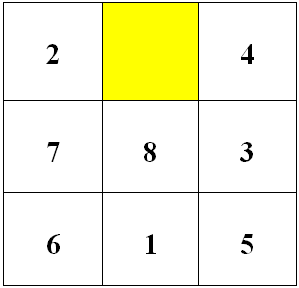
\includegraphics[height=3in]{Example}
    \else
      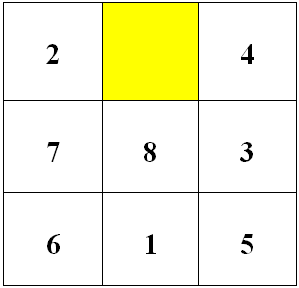
\includegraphics[bb = 92 86 545 742, height=6in]{Example}
    \fi
    \caption{Trạng thái ví dụ}
    \label{FigAir}
  \end{center}
\end{figure}
Xét ô thứ nhất có giá trị 2: Phía sau có 1 ô nhỏ hơn (1) => n1 = 1\\
Xét ô thứ ba có giá trị 4: Phía sau có 2 ô nhỏ hơn (3,1) => n3 = 2\\
Xét ô thứ tư có giá trị 7: Phía sau có 3 ô nhỏ hơn (3,6,1,5) => n4 = 4\\
Xét ô thứ năm có giá trị 8: Phía sau có 4 ô nhỏ hơn (3,6,1,5) => n5 = 4\\
Xét ô thứ sáu có giá trị 3: Phía sau có 3 ô nhỏ hơn (6,1,5) => n6 = 3\\
Xét ô thứ bảy có giá trị 6: Phía sau có 2 ô nhỏ hơn (1,5) => n7 = 2\\
Xét ô thứ tám có giá trị 1: Phía sau không còn ô nào nhỏ hơn => n8 = 0\\\\
Như vậy ta có công thức tính N như sau: \\
\bfseries N = 1 + 2 + 4 + 4 + 3 + 2 + 0 = 16\\
\mdseries Ta có 16 mod 2 = 0 => Trường hợp này bài toán có thể đưa về trạng thái đích.\\
\\
Những trạng thái của bảng số mà có thể chuyển về trạng thái đích gọi là cấu hình hợp lệ, ngược lại gọi là cấu hình không hợp lệ.\\
Đây là kết quả mà ta mong muốn:\\
\begin{figure}[!htbp]
  \begin{center}
    \leavevmode
    \ifpdf
      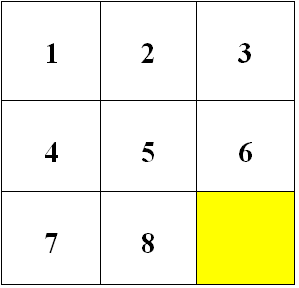
\includegraphics[height=3in]{GoalState}
    \else
      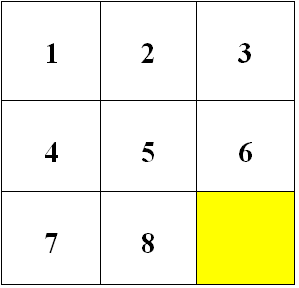
\includegraphics[bb = 92 86 545 742, height=6in]{GoalState}
    \fi
    \caption{Trạng thái đích}
    \label{FigAir}
  \end{center}
\end{figure}

%\cite.









